\setcounter{subsection}{0} 
\part{Chapters subdivision}
\paragraph{Introduction:} the Chapter 1 describes the properties of the anti-neutron and its detection techniques in the high-energy physics (HEP) context. Its primary interactions -such as annihilation and hadronic shower production- are then exploited, discussing some hadronic models very quickly. The MANTRA (Measuring Anti-Neutron: Tagging and Reconstruction Algorithm) project is then described as a method to measure anti-neutron energies up to 10 GeV using an electromagnetic calorimeter.

\paragraph{The Belle II experiment:} the Chapter 2 provides an overview of the SuperKEKB accelerator and Belle II detector. In the context of $\bar{n}$ studies, the Electromagnetic Calorimeter (ECL) plays a key role in hadron detection; a detailed discussion about the ECL is thus provided, covering the description of its inorganic crystals and the explanation of the clustering algorithm. The ECL performance are then discussed.


\paragraph{The Belle II Analysis Software Framework:} the Chapter 3 introduces the the Belle II Analysis Software Framework (basf2), providing an overview of its operation method and its role in the Monte Carlo simulation and reconstruction processes at Belle II experiment. Then, the Topology Analysis (TopoAna) independent software is described, concluding with the introduction of the Belle II Grid.


\paragraph{The ECL reconstruction:} the Chapter 4 provides a detailed description of the ECL clustering algorithm and analyzes ECL energy performance, followed by the definition of shower cluster variables.

\paragraph{Study of the Monte Carlo signal channel:} the Chapter 5 is devoted to the study of the kinematic variables of anti-neutrons $\bar{n}$, including momentum, angular distributions and related observables. The analysis follows a semi-exclusive approach over the selected channel $e^+ e^- \rightarrow p \pi^-  \bar{n}$, studying both cases with and without Initial State Radiation (ISR) reconstruction, where the recoil system is made of  $p  \pi^-  (\gamma_{ISR})$. Therefore, the recoil system variables are compared to those of the anti-neutrons candidates, studying the response of a Kinematic Fit as well. 
$\\$
Cluster split-off and pre-showering effects are investigated studying anti-neutrons relatives chain. Several neutral cluster variables associated to anti-neutron candidates are then described and studied for both ISR and NO ISR cases, including the analysis of their relatives contributions.

\paragraph{Study of the Monte Carlo cocktail production:} the Chapter 6 introduces the study of the channel of interest within the entire $q\bar{q}$ cocktail production. First, the possible Belle II processes are introduced, along with the typical cross sections that characterize them, and their contributions to the recoil mass distribution are discussed. Further selections from the previous analysis are then discussed, including a stricter selection on the reconstructed $\bar{n}$ direction based on a Performance Metric figure-of-merit study. Subsequently, the sideband method is applied to the reconstructed $\bar{n}$ cluster variables, evaluating the feasibility of subtracting the background contribution from the signal.

\paragraph{Data - Monte Carlo comparison:} the Chapter 7 finalizes the analysis by performing a Data/MC agreement between the cluster variables obtained from the $q\bar{q}$ cocktail and those from real data.

\newpage
\setcounter{subsection}{0} 
\part{Introduction}
The Standard Model is one of the greatest achievements of modern science, especially in the field of high-energy particle physics. Its reliability is the result of a long process that began in the 20th century and received its definitive confirmation in 2012 with the discovery of the Higgs boson. 
$\\$
However, there are some topics which remain unsolved, like the non-trivial neutrino mass or the presence of dark matter on cosmological scales. The Standard Model still represents an excellent phenomenological description of subatomic processes, up to the TeV energy scale.
$\\$
In this framework, the Belle II experiment, located at the SuperKEKB facility, plays a fundamental role in exploring scenarios that go beyond the standard physics, thus entering the so-called \emph{new physics}.
$\\$
In parallel with experiments that maximize the energy, the aim of Belle II is to explore the intensity frontier, investigating scenarios of high instantaneous luminosity up to $8 \times10^{35} cm^{-2} s^{-1}$, around (and not limited to) the $\Upsilon(4S)$ resonance energy. 
$\\$
This approach enables flavour physics studies of heavy mesons such as B mesons, searching for very rare processes and facilitating the identification of potential discrepancies with Standard Model predictions and opening the door to Beyond Standard Model physics.

\subsection{The B Factories}
Since the end of the XX century, two asymmetric-energy $e^+e^-$ B factories -KEKB for the Belle experiment at KEK and PEP-II for the BaBar experiment at SLAC- have achieved huge success, confirming the Standard Model in the quark flavour sector, establishing the presence of CP violation in the B meson system through the decay process $B^0 (\bar{B}^0) \rightarrow J/\Psi K_S^0$ \cite{Abe:2001sin2phi,Abe:2002largeCP,Aubert:2001B0CP,Aubert:2002timeCP}. This result fixed the main target of the present B factories. Experimental results confirm that the Kobayashi–Maskawa mechanism, a key component of the Standard Model of elementary particles, is the dominant source of CP violation observed in nature.
$\\$
The Belle experiment proved its ability to measure a number of decay modes of the B meson and to extract Cabibbo-Kobayashi-Maskawa (CKM) matrix elements and other interesting observables. Precise measurements and new observations from Belle have overconstrained the quark flavor sector of the Standard Model. This sector remains self-consistent within the current experimental precision.
$\\$
However, several fundamental questions persist in the quark and lepton flavor sectors; the Standard Model requires numerous parameters, including quark and lepton masses and mixing angles that must be determined experimentally.
$\\$
Furthermore, from a cosmological perspective, the matter-antimatter asymmetry of the Universe poses a great challenge. While the CP violation constitutes one of the necessary conditions for the evolution of a matter-dominated Universe \cite{Sakharov:1967}, its magnitude cannot be explained solely by the CP violation within the Standard Model, which originates from quark mixing.
$\\$
Exploring such scenarios requires substantial luminosity at present B factories. The SuperKEKB B Factory has been designed to investigate the physics of B mesons processes. Due to the very large production cross section of $b$-quarks in hadron collisions, certain measurements such as $B_s\rightarrow\mu\mu$ can be performed more effectively at hadron colliders, such as LHC. However, $e^+e^-$ machines provide a much cleaner environment, essential for precision observables involving photons, $\pi^0$'s, $K_L^0$'s, or neutrinos in the final state.
$\\$
At the $\Upsilon(4S)$ resonance, $B\bar{B}$ pairs are produced near threshold without associated particles. By fully reconstructing the four-momentum of one $B$ ($\bar{B}$) meson from its decay products (full reconstruction technique), the missing momentum of the other $\bar{B}$ ($B$) meson decay can be inferred. This technique is essential for measuring channels with neutrinos in the final state. Therefore, SuperKEKB undoubtedly complements hadron collider experiments from both theoretical motivation and experimental perspectives.


\subsection{Anti-neutron in HEP physics}
The anti-neutron $\bar{n}$ ($\bar{u} \bar{d} \bar{d}$) is the anti-particle of the neutron n ($udd$), neutral hadron of mass 0.939565 $GeV/c^2$ and spin $\frac{1}{2}$, with magnetic moment of $1.91 \mu_N$, where  $\mu_N$ is the nuclear magneton. Its existence was expected by the principle of invariance under charge conjugation and experimentally proved in 1956 \cite{cork1956}, one year after the anti-proton $\bar{p}$ \cite{chamberlain1955}.
$\\$
The anti-neutron plays a key role in several physics measurements, both in collider physics and in astrophysical contexts. Since it is electrically neutral, it cannot be easily observed directly, allowing its detection via the products of its annihilation with ordinary matter.
$\\$
For example, the measurement of the neutron electromagnetic form factor in the time-like region is strongly affected by the performance of the $\bar{n}$ detection. The BESIII experiment has shown \cite{ablikim2021} an oscillating behaviour in the electromagnetic structure of the neutron in the study of the $e^+e^- \rightarrow n\bar{n}$ annihilation process. Direct detection of the $\bar{n}$ would further refine this analysis by enabling a more proper identification of the final state.
$\\$
Another example, where an improved direct measurement of the $\bar{n}$ would significantly enhance the studies, is the analysis of hyperon decay channels at B factories (and beyond). Some possible decay channels where the $\bar{n}$ is the only unreconstructed particle in the final state are shown below:

	\begin{center}
		$\bar{\Lambda}^0 \rightarrow \pi^0 + \bar{n}$, \hspace{1cm} $\bar{\Sigma}^- \rightarrow \pi^- + \bar{n}$, \hspace{1cm} $\bar{\Lambda}_c \rightarrow  K_s^0 + \pi^0 +\bar{n} $
	\end{center}

Furthermore, the anti-deuteron $\bar{D}$ hadronization is commonly described by a coalescence mechanism \cite{serk2022}, where a $\bar{p}$ and a $\bar{n}$ sufficiently close in phase space bind to form a $\bar{D}$. The latter is expected among the products of dark matter annihilation \cite{donato2000}. Thus, improved $\bar{n}$ detection would enhance the simultaneous measurement of the $\bar{n}$–$\bar{p}$ correlation function in $\bar{D}$ production, providing deeper insight into dark matter distributions.
$\\$
GEANT4 is the main toolkit designed for simulating the passage of particles through matter \cite{geant4_cds}. It finds applications across high-energy, nuclear and accelerator physics, as well as in medical and space science research. A deeper knowledge on anti-neutrons kinematic and interaction would improve also Monte Carlo GEANT4 models of the hadronization process. This requires better $\bar{n}$ reconstruction, which remains challenging in standard HEP experiments.

\subsubsection{Anti-neutron interactions in physics}
Due to isospin symmetry, before the 1980s, it was believed that anti-neutron strong interactions with nucleons ($N$) and matter would provide no additional information beyond anti-proton results. For anti-protons obtain proper beams was much easier.
$\\$
The experimental landscape underwent a significant transformation in the mid-1980s with the development of dedicated anti-neutron beams, which enabled the observation of unique $\bar{n}$ characteristics, such as:

\begin{itemize}
\item The anti-nucleon nucleon $\bar{N}N$ interaction, in $\bar{p}p$ interactions, is a mixture of isospin $I=0$ and $I=1$ amplitudes, while the $\bar{n}p$ is a pure $I=1$ eigenstate. The same difference between $\bar{p}p$ and $\bar{p}n$ interactions could be obtained by means of the charge-symmetric system $\bar{p}n$ copiously produced at deuterium target experiments. However, the use of deuterium introduces several drawbacks, such as re-scattering effects that may largely distort the final spectra \cite{eastman1973}. This effect is absent if the $\bar{N}N$ system with pure $I=1$ is formed by $\bar{n}$ interactions on protons of the material.
\item The $\bar{n}p$ interaction is a pure strong interaction, since it is free from Coulomb corrections, that are necessarily present in the $\bar{p}p$ interaction and may introduce further complications and ambiguities in the analysis of the data, especially at low-momenta.
\item At low momentum, typically below 1 GeV/c,  only S- and P-waves are present in the elementary $\bar{n}p$ interaction, described by the Dover-Richard parametrization \cite{bressani2003}. Fig.~\ref{fig:DoverRichard} shows the trends of S-wave and P-wave annihilation cross sections according to the Dover-Richard parametrization, where in $\bar{n}p$ interactions the S-wave contribution diminishes with increasing energy, whereas the P-wave contribution grows \cite{dover1992, ueda1979}.
\end{itemize}

\begin{figure}[H]
    \centering
    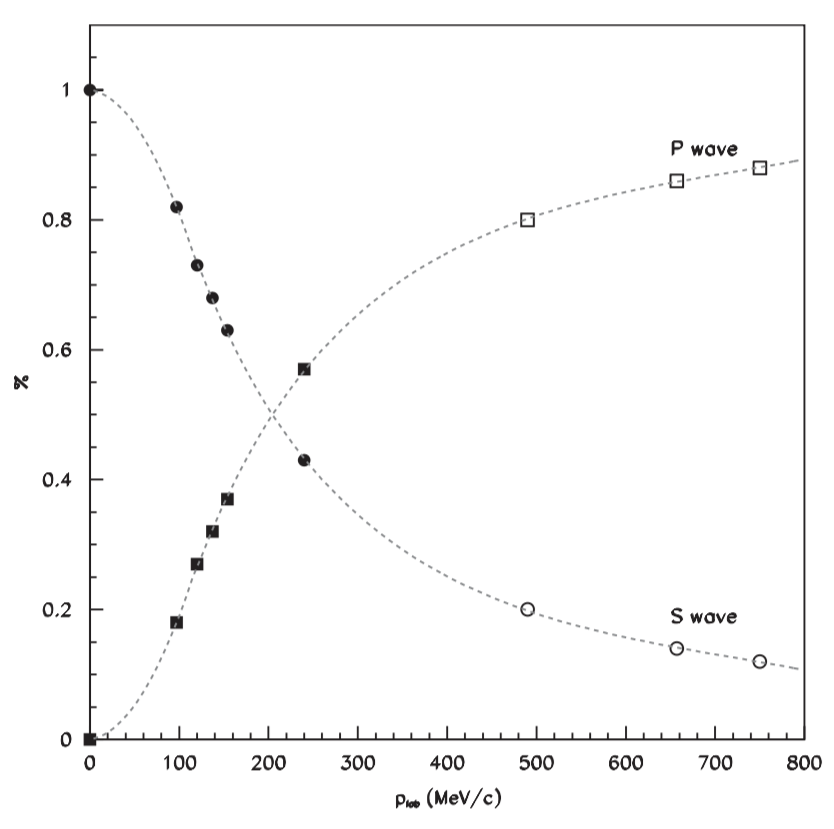
\includegraphics[width=0.70\textwidth]{nbar_exp/images/DoverRichard}
    \caption{Trends of S- and P-wave annihilation cross sections according to annihilation models: the full markers (circles for S-wave, squares for P-wave) are from the Dover–Richard model, while the open ones have been obtained by using a version of the optical model.}
    \label{fig:DoverRichard}
\end{figure}
Therefore, the $\bar{n}p$ system can be represented as an isospin eigenstate $|I, I_3\rangle = |1, +1\rangle$. It is not a C-parity eigenstate, then only J (total angular momentum), P (spatial parity) and G-parity are good quantum numbers, where G-parity is defined as the combination of charge conjugation and a rotation of $180^\circ$ in isospin space as $G = C\,e^{i\pi I_2}$.
$\\$
Since $\bar{n}p$ is an antifermion-fermion system, the following equations can be obtained:
\begin{center}
$P = (-1)^{L+1}$ \hspace{0.3cm} $G = (-1)^{L+S+1}$ 
\end{center}
where L is the relative angular momentum between the anti-neutron and the proton, while S is the spin of the system, namely 0 or 1. The $I^G(J^P)$ quantum numbers allowed for the lowest initial states are shown in Tab.~\ref{tab:q_number}.
\begin{table}[h]
  \centering
  \begin{tabular}{llll}
    \hline
    Wave & ${}^{2S+1}L_J$ & $I^G(J^P)$ \\
    \hline
    % S-wave
    S & ${}^{1}S_{0}$ & $1^{-}(0^{-})$ \\
      & ${}^{3}S_{1}$ & $1^{+}(1^{-})$ \\
    \hline
    % P-wave
    P & ${}^{1}P_{1}$ & $1^{+}(1^{+})$ \\
      & ${}^{3}P_{0}$ & $1^{-}(0^{+})$ \\
      & ${}^{3}P_{1}$ & $1^{-}(1^{+})$ \\
      & ${}^{3}P_{2}$ & $1^{-}(2^{+})$ \\
    \hline
    % D-wave
    D & ${}^{1}D_{2}$ & $1^{-}(2^{-})$ \\
      & ${}^{3}D_{1}$ & $1^{+}(1^{-})$ \\
      & ${}^{3}D_{2}$ & $1^{+}(2^{-})$ \\
      & ${}^{3}D_{3}$ & $1^{+}(3^{-})$ \\
    \hline
  \end{tabular}
  \caption{Quantum numbers $I^G(J^P)$ on $S$, $P$ e $D$ waves.}
  \label{tab:q_number}
\end{table}
$\\$
Even if the total cross section $\sigma_T$ is the first piece of information on the interaction between to particles, for the case $\sigma_T(\bar{n}p)$ could be tough to measure it. The final value of $\sigma_T$ published in \cite{armstrong1987} shows how the data could be fitted to a simple parametrization \cite{bertin1997}, obtaining the results showed in Fig.~\ref{fig:cross_section}.
\begin{figure}[h]
    \centering
    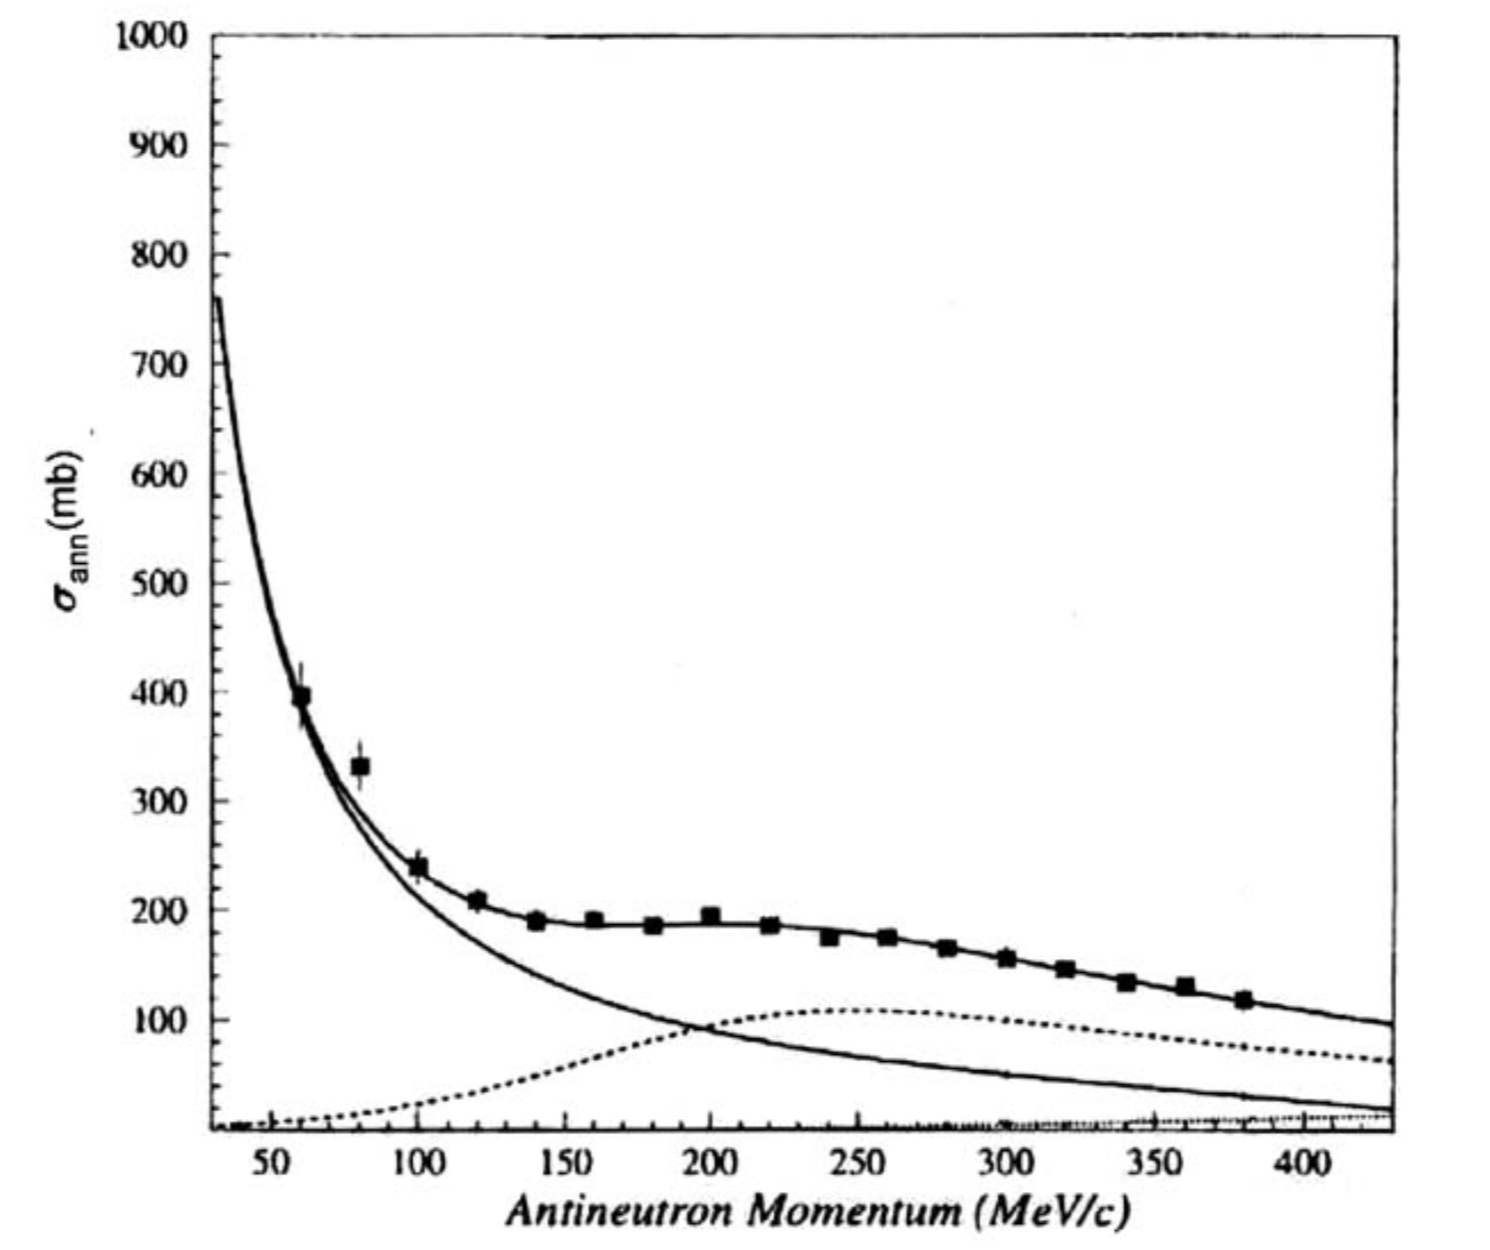
\includegraphics[width=0.55\textwidth]{nbar_exp/images/cross_section}
    \caption{Fit of the annihilation cross section $\sigma_{ann}(\bar{n}p)$, measured by OBELIX up to 400 MeV/c, including S (solid line), P (dashed line) and D (dotted line) wave contribution.}
    \label{fig:cross_section}
\end{figure}

\subsubsection{The anti-nucleon–nucleon interaction}
The first approach to describe the antinucleon-nucleon ($\bar{N}N$) interaction relies on interaction models. Unlike Quantum ElectroDynamics (QED), where the coupling constant $\alpha$ grows with energy and diverges at finite energy, asymptotic freedom characterizes the  Quantum ChromoDynamics (QCD), the quantum field theory of the strong force between quarks and gluons. Quarks interact weakly at high energies, enabling perturbative calculations, but at low energies the interaction strengthens dramatically, confining quarks and gluons within composite hadrons. Here, the divergent coupling constant $\alpha_s$ renders perturbative approaches invalid, making interaction models essential for describing strong interactions in the $\lesssim 1$ GeV energy range.
$\\$
The core of this approach is that, following the $\bar{N}N$ annihilation, a \emph{fireball} (which represents the $\bar{N}N$ system) with definite energy and volume $\Omega = \frac{4}{3}\pi R_0^3$ is formed, where $R_0 \sim 1$ fm is the nucleon radius. All the possible $\bar{N}N$ annihilation final states -primarily light mesons- may be reached through the decay of the fireball, according to the statistical Fermi model, where the probability of a final state is determined solely by the available phase space \cite{fermi1950}.
$\\$
The use of interaction models in $\bar{N}N$ interaction generally allows a correct description of annihilation, even if it doesn't reproduce the whole experimental scenario, such as differences between nucleon and anti-nucleon scattering and stopping power (Barkas effect) \cite{barkas1957}. The reason why it happens is the that the potential formulation used to describe the short range interactions (where annihilation plays the most important role) is not sensitive to the details of the internal dynamics, namely the interactions between quarks and gluons.
$\\$
The second approach is the Effective Range (ER) expansion one, which is independent on any hypothesis concerning the interaction potential and it is based on the obtained fit of experimental cross sections \cite{mahalanabis1988}. The annihilation cross section for two interacting particles may be expressed as a partial waves expansion as follows:
\begin{center}
$\sigma_{\text{ann}} = \sum_{L} \sigma^{\text{ann}}_{L} = \frac{4\pi}{k^{2}} \sum_{L} (2L + 1)\left(\Im m f_{L} - |f_{L}|^{2}\right)$,
\end{center}
where $k$ is the center-of-mass momentum of the incident particle, and the partial amplitude $f_L$ may be written as a function of the $\delta_L$ wave phase shifts induced by the interaction in the system wave function:
\begin{center}
$f_L = \frac{1}{cot\delta_L - i}$,
\end{center}

The partial waves may be expanded as a series in $k$, following the so-called \emph{Effective Range (ER) expansion formalism}:
\begin{center}
$k^{2L+1} \cdot cot\delta_L = \frac{1}{A} + \rho k^2 + O(k^4)$,
\end{center}
where A is the scattering length, and $\rho$ is the interaction range. For S and P partial waves can be obtained:
\begin{center}
$k \cdot cot\delta_0 = \frac{1}{a} + \frac{1}{2} r k^2$ \\
\vspace{0.3cm}
$k^3 \cdot cot\delta_1 = \frac{1}{b} - \frac{3}{2} \frac{1}{R} k^2$
\end{center}
$a$ and $b$ are, respectively, the scattering length and the nucleon volume, while $r$ and $R$ are the two effective ranges for the two partial waves. These parameters must be determined by a phenomenological fit to the annihilation cross section data. For example, for the $I=1$ case, relevant to the $\bar{n}p$ interaction case, it was found that \cite{bertin1997}:
\begin{center}
$a_1 = (0.4 + 0.5 i)$ fm and $r_1 = (-1.4 + 1.8 i)$ fm for S-wave, \\
\vspace{0.3cm}
$b_1 = (0.8 + 0.1i)$ fm$^3$ and $R_1 = (0.2 - 0.4 i)$ fm for P-wave
\end{center}

\subsubsection{Electromagnetic and hadronic showers}
In the energy scenario beyond 10 MeV, bremsstrahlung and pair production are the main processes which respectively involve electrons/positrons and photons, leading to the development of electromagnetic showers within the material. Therefore, to detect such phenomena, HEP experiments employ electromagnetic calorimeters. The electromagnetic calorimeter is a device whose size and density are designed to fully contain the electromagnetic shower, producing a signal proportional -or at least correlated- to the energy of the incident particle that initiated the shower. Since the radiation length $X_0$ (defined as the distance over which a high-energy electron loses $1/e$ of its energy through bremsstrahlung) determines the size of the electromagnetic shower, the typical longitudinal size for these detectors is of the order of 10-20 $X_0$ ($\sim 20-40$cm).
$\\$
Furthermore, hadronic showers can be originated from strong interactions of high energy (beyond $\sim GeV$) hadrons, such as protons, neutrons and pions, with the material. To detect this kind of showers, a hadronic calorimeter may be employed; since the interaction length $\lambda$ determines the hadronic shower size and $\lambda >> X_0$, hadronic showers are larger and longer than electromagnetic ones, requiring hadronic calorimeters to be significantly bigger than electromagnetic calorimeters. Therefore, homogeneous calorimeters cannot be used for hadronic calorimetry as they are for electromagnetic calorimetry. Instead, the sampling calorimeter technique is mandatory, employing alternating layers of passive, dense absorber material and active detection material.
$\\$
For example, approximately 95\% of a hadronic shower is contained within a cylinder of radius equal to the hadronic interaction length ($\lambda_{had} \simeq 44.1$ cm, in CsI(Tl)). In contrast, about 90\% of an electromagnetic shower is contained within a cylinder defined by the Molière radius ($R_M \simeq 3.6$ cm in CsI(Tl)). Therefore, there is an order of magnitude difference between the two values. A shape comparison between these two type of shower can be observed in Fig.~\ref{fig:shower_comp}.

\begin{figure}[H]
    \centering
    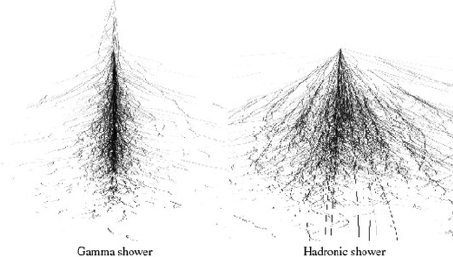
\includegraphics[width=0.60\textwidth]{nbar_exp/images/gamma_vs_hadronic}
    \caption{Electromagnetic shower vs hadronic shower comparison.}
    \label{fig:shower_comp}
\end{figure}

The $\bar{n}$ primarily interacts via the strong nuclear force, annihilating with nucleons in the material ($\sigma \sim 100$ mb), mainly producing light mesons such as pions which subsequently interact within the calorimeter:
	\begin{center}
		$\bar{n} + p/n \rightarrow \pi^{\pm}, \pi^0 ..$
	\end{center}
	
The $\pi^0$ meson mainly ($\sim 98.8 \%$) decays into a couple $\gamma \gamma$, producing electromagnetic showers that are fully contained in the calorimeter.
$\\$
While charged pions $\pi^+$ and $\pi^-$ undergo both electromagnetic and hadronic interactions, producing final products that are not fully contained within the calorimeter volume, this leads to a lack in the energy deposited in the detector. Both forward and backward directions are then involved, according to the reaction kinematics.

\subsection{The MANTRA Project}
It may be challenging for general-purpose experiments to directly identify and reconstruct anti-neutrons produced in $e^+e^-$ collisions, such as those at Belle II and BESIII, which lack a hadronic calorimeter. Anti-neutrons generally annihilate with detector material nucleons such as that of an electromagnetic calorimeter, producing hadronic showers which only allows a loose measurement of the anti-neutron energy with extremely large uncertainty.
$\\$
Since anti-neutron kinematics have so far been measured via missing mass methods or isospin symmetry with anti-protons, a direct anti-neutron reconstruction would be highly  desirable, especially in studying processes with neutral hadrons, such as $B^+ \rightarrow K^+ n \bar{n}$ or $J/\Psi \rightarrow p \pi^- \bar{n}$.
$\\$
This thesis fits in the larger context of the MANTRA (Measuring Anti-Neutron: Tagging and Reconstruction Algorithm) PRIN2022 project, an inter-university (University of Turin and University of Ferrara) and INFN effort aimed at developing a method to improve the reconstruction of anti-neutron in existing high-energy physics experiments. It provides a general approach to measure the energy of anti-neutrons $\bar{n}$ up to 10~GeV using an electromagnetic calorimeter. The main idea is to combine the information from a high time-resolution time of flight detector (TOP and TOF in the Belle II and in the BESIII experiments, respectively) with that from an electromagnetic calorimeter (ECL and EMC in the Belle II and in the BESIII experiments, respectively), where the anti-neutrons annihilation occurs.
$\\$
Due to its neutral charge and its immediate annihilation, tagging $\bar{n}$ can be very challenging. However, the annihilation can produce self-contained light mesons, mostly made of high-energy pions ($\pi^-, \pi^0, \pi^+$) and soft nuclear fragments. These can be detected in the Electromagnetic Calorimeter (detailed examination in the next chapter), where charged pions can produce hadronic showers, while neutral pions immediately decay into two photons which produce electromagnetic showers in the calorimeter volume. The comparison of the cluster energy deposition patterns, the so called shower shapes variables, left in the ECL by anti-neutrons and other neutral particles, such as photons, can improve the characterization of neutral particles.
$\\$
A crucial aspect of the analysis process is the role of simulation, where GEANT4 \cite{geant4_cds} (more details in the next chapter) plays a central role, modeling the hadronic interactions in the calorimeter; realistic simulation is essential to accurately reproduce real data. For $\bar{n}$ annihilation, parameterizations are typically derived from $\bar{p}$ measurements, necessitating validation against data.
$\\$
This thesis aims to study the $\bar{n}$ hadronic interactions modeled by simulation software and compare them with those observed in Belle II data, focusing exclusively on signals from the Belle II electromagnetic calorimeter. To achieve this, $\bar{n}$ variables are first studied using a signal sample, where only the specifically selected processes with $\bar{n}$ in the final state are generated. Several background channels are then included to simulate the complete Belle II environment, concluding with a comparison between the results obtained from simulations and those from real data, with a Data/MC agreement.
$\\$
Therefore, this work addresses the following question:

\begin{center}
\textbf{Are $\bar{n}$ hadronic showers correctly simulated in the Belle II software?}
\end{center}
